% PLOS journals, following PLOS's own LaTeX template (plain article class; the
% only file used from it is plos2025.bst).
% Differences from PLOS's template, kept deliberately small:
%   - natbib (numbers) replaces the cite package, so the shared text's \citep
%     works unchanged. The output is the same numbered Vancouver style.
%   - Section numbering is switched off here, not by rewriting paper.tex.
%   - Figures are not included: PLOS wants captions in the text and the image
%     files uploaded separately (the bundle renames them Fig1.tif, ...).
\documentclass[10pt,letterpaper]{article}
\usepackage[top=0.85in,left=2.75in,footskip=0.75in]{geometry}
\usepackage[numbers,sort&compress]{natbib}
% Packages the main text relies on. Every main-text wrapper loads this straight
% after its \documentclass, then adds only what that version needs.
%
% Keep this list short. Journal systems re-compile the source with their own,
% often older, TeX installations, and pandoc (for .docx) understands only
% standard LaTeX. natbib is loaded by each wrapper, because some journal
% classes load it themselves with their own options.
\usepackage{amsmath,amssymb}
\usepackage{graphicx}
\usepackage{booktabs}
\graphicspath{{figures/}}

% \linelabel comes from lineno, which not every version loads.
\AtBeginDocument{\providecommand{\linelabel}[1]{}}

% Notation shortcuts only. Every macro here must be a plain \newcommand that
% expands to standard LaTeX math, so pandoc can expand it for .docx output.
\newcommand{\R}{\mathbb{R}}
\newcommand{\E}{\mathbb{E}}
\newcommand{\dd}{\mathrm{d}}
\newcommand{\vect}[1]{\mathbf{#1}}


% Title, authors, abstract and statements. Each wrapper sets the author lists
% by defining \paperauthor, \correspondingauthor and \paperaffiliation.
% Everything about the paper except the main text: title, authors, abstract
% and back-matter statements. Every version reads this file and sets it in its
% own style, so this is the only place to edit them.

\newcommand{\papertitle}{A single-source LaTeX template for computational biology papers}
\newcommand{\papershorttitle}{Single-source paper template}
\newcommand{\papershortauthors}{Author et al.}
\newcommand{\paperkeywords}{LaTeX, BibTeX, journal submission, preprints}

% Authors, in order. Mark any number of corresponding authors.
%   \paperauthor{Given}{Family}{affiliation numbers}
%   \correspondingauthor{Given}{Family}{affiliation numbers}{email}
\newcommand{\paperauthors}{%
  \correspondingauthor{First}{Author}{1}{first.author@example.org}%
  \paperauthor{Second}{Author}{1,2}%
}

%   \paperaffiliation{number}{Department}{Institution}{City}{Country}
\newcommand{\paperaffiliations}{%
  \paperaffiliation{1}{Department}{Institution}{City}{Country}%
  \paperaffiliation{2}{Department}{Institution}{City}{Country}%
}

% One paragraph, no citations: most journals forbid them in the abstract.
\newcommand{\paperabstract}{%
This document is both the example paper and the documentation for a LaTeX
template. It is written once and built as a styled preprint, a review copy
with line numbers, a supplement and journal submissions whose source is plain
LaTeX in each journal's own format. The abstract, like the title, authors and
statements, is written once in \texttt{metadata.tex}; replace this text with
your own, keeping to one paragraph without citations.}

\newcommand{\paperacknowledgements}{%
Statements such as this one are written once in \texttt{metadata.tex} and
placed wherever, and under whatever heading, each version needs them.}

\newcommand{\paperfunding}{%
Funding statement, for example: This work was supported by [funder]
[grant number].}

\newcommand{\papercompeting}{%
Competing interests statement, for example: The authors declare no competing
interests.}

\newcommand{\paperavailability}{%
Data and code availability statement, for example: Code to reproduce the
analyses is available at [repository URL].}

\newcommand{\papercontributions}{%
Author contributions statement, for example using CRediT roles.}


% Labels from the supplement (all prefixed S:), extracted by the Makefile from
% build/supplement.aux, so the main text can write \ref{S:fig:growth}.
% Submission bundles replace these references with plain numbers.
\input{build/supp-labels}

\usepackage{changepage}
\usepackage{textcomp,marvosym}
\usepackage{nameref,hyperref}
\usepackage[right]{lineno}
\usepackage[nopatch=eqnum]{microtype}
\DisableLigatures[f]{encoding = *, family = * }
\usepackage[aboveskip=1pt,labelfont=bf,labelsep=period,justification=raggedright,singlelinecheck=off]{caption}
\usepackage{lastpage,fancyhdr}

\raggedright
\setlength{\parindent}{0.5cm}
\textwidth 5.25in
\textheight 8.75in
\renewcommand{\figurename}{Fig}
\setcounter{secnumdepth}{0}
\bibliographystyle{plos2025}
\makeatletter
\renewcommand{\@biblabel}[1]{\quad#1.}
\makeatother
\renewcommand{\includegraphics}[2][]{}

\pagestyle{fancy}
\fancyhf{}
\rfoot{\thepage/\pageref{LastPage}}
\renewcommand{\headrulewidth}{0pt}
\renewcommand{\footrule}{\hrule height 2pt \vspace{2mm}}
\fancyheadoffset[L]{2.25in}
\fancyfootoffset[L]{2.25in}
\lfoot{\today}

% PLOS sets authors as a run of names with superscript affiliations, and
% lists corresponding authors' emails after the affiliations.
\makeatletter
\def\plos@sep{}
\def\plos@emails{}
\newcommand{\paperauthor}[3]{\plos@sep#1 #2\textsuperscript{#3}\def\plos@sep{, }}
\newcommand{\correspondingauthor}[4]{%
  \plos@sep#1 #2\textsuperscript{#3*}\def\plos@sep{, }%
  \g@addto@macro\plos@emails{\plos@esep#4\def\plos@esep{, }}}
\newcommand{\paperaffiliation}[5]{\textbf{#1} #2, #3, #4, #5\\}
\newcommand{\paperemails}{{\def\plos@esep{}\plos@emails}}
\makeatother

\begin{document}
\vspace*{0.2in}

\begin{flushleft}
{\Large
\textbf{\papertitle}
}
\newline
\\
\paperauthors
\\
\bigskip
\paperaffiliations
\bigskip
* \paperemails
\end{flushleft}

\section*{Abstract}
\paperabstract

\section*{Author summary}
PLOS asks for a plain-language summary for non-specialists (150--200 words).
Only PLOS uses one, so it is written in \texttt{journals/plos/plos.tex} rather
than in \texttt{metadata.tex}.

\linenumbers

% The main text, shared by every version. Title, authors, abstract and the
% back-matter statements are in metadata.tex. Keep Methods as a single
% \section{Methods}: the Nature build moves that section to the end.

\section{Introduction}\label{sec:intro}

This is the template's example paper. Each part of it, from the sections,
equations, figure and table to the citations and references into the
supplement, is here to show a feature, and the text explains how that feature
is written and built. Replace it with your own paper.

A paper is now read in several forms: a preprint, a copy with line numbers for
co-authors and reviewers, and one or more journal submissions. Most journals
accept almost any PDF at first submission, but at acceptance they want editable
source, in practice LaTeX \citep{lamport1994} or Word. The template therefore
keeps a single LaTeX source and builds every version from it, with each
journal's formatting kept out of the text.

\section{Methods}\label{sec:methods}

\subsection{Source files}

The writing lives in three files. \texttt{metadata.tex} holds the title,
authors, affiliations, abstract and statements; \texttt{paper.tex} holds this
text; and \texttt{supplement.tex} holds the supplementary information.
References are kept in \texttt{refs.bib} and cited by key, with BibTeX
formatting them in each journal's style \citep{patashnik1988}. Figures are
produced elsewhere and copied into \texttt{figures/} as finished files.

\subsection{Building each version}

Each version has a short wrapper that sets the document class and layout,
defines how the authors in \texttt{metadata.tex} are set in that class, and
includes the shared text. Running \texttt{make} compiles each wrapper with
pdfLaTeX and BibTeX (Fig.~\ref{fig:pipeline}). For a journal it can also make
a submission bundle: the wrapper flattened into one file with the bibliography
pasted in and references into the supplement written as plain numbers,
together with the figures and the journal's class files. The Nature build
moves this Methods section after the Discussion, as Nature Portfolio journals
require, which is why Methods must stay a single section.

\subsection{Equations}

Equations use standard \texttt{amsmath} environments and are numbered in every
version. For example, the logistic model of population growth
\citep{verhulst1838} is
\begin{equation}
  \frac{\dd N}{\dd t} = r N \left(1 - \frac{N}{K}\right),
  \qquad N(0) = N_0 ,
  \label{eq:logistic}
\end{equation}
where $r$ is the growth rate and $K$ the carrying capacity. Equation~\eqref{eq:logistic}
has the solution
\begin{equation}
  N(t) = \frac{K}{1 + \left(K/N_0 - 1\right) e^{-r t}} .
  \label{eq:solution}
\end{equation}
Notation shortcuts such as the upright differential in
Eq.~\eqref{eq:logistic} are defined once in \texttt{macros.tex}.

\section{Results}\label{sec:results}

Figure~\ref{fig:pipeline} shows how the source files become the finished
versions, and Table~\ref{tab:versions} compares the example versions. Tables
use \texttt{booktabs} rules, and the grouped column headings show that
spanning columns survive every build.

\linelabel{rev:linelabels}A sentence can be marked with a line label, which
lets a response to reviewers quote its line number in the review copy. The
main text can also refer into the supplement: an example data figure is
Supplementary Fig.~\ref{S:fig:growth}, and Supplementary
Note~\ref{S:sec:crossrefs} explains how references between the two documents
are resolved.

\begin{figure}[tbp]
  \centering
  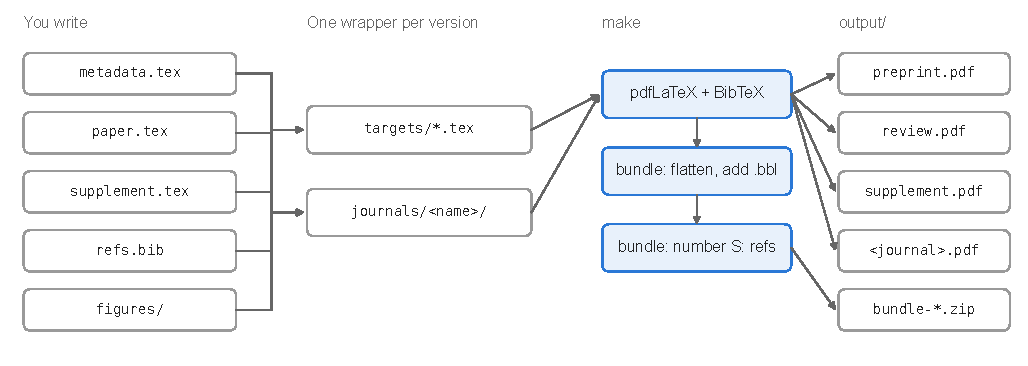
\includegraphics[width=\linewidth]{pipeline}
  \caption{\textbf{From source files to finished versions.} The shared text
    and metadata are included by one wrapper per version, which
    \texttt{make} compiles. Submission bundles are also flattened into a
    single file with the bibliography and supplementary numbers written in.
    Everything finished goes to \texttt{output/}.}
  \label{fig:pipeline}
\end{figure}

\begin{table}[tbp]
  \centering
  \caption{\textbf{How the example versions differ.} The text is identical in
    all of them.}
  \label{tab:versions}
  \begin{tabular}{lllll}
    \toprule
            & \multicolumn{2}{c}{Layout} & \multicolumn{2}{c}{Citations} \\
    \cmidrule(lr){2-3}\cmidrule(lr){4-5}
    Version & Line numbers & Figures & Style & Order \\
    \midrule
    Preprint       & No  & In text  & Numbered    & Citation \\
    Review         & Yes & In text  & Numbered    & Citation \\
    Nature         & Yes & In text  & Numbered    & Citation \\
    PLOS           & Yes & Separate & Vancouver   & Citation \\
    Bioinformatics & Yes & In text  & Author--year & Alphabetical \\
    \bottomrule
  \end{tabular}
\end{table}

\section{Discussion}\label{sec:discussion}

The template trades a few conveniences for portability. Citations are made
with one command so that numbered and author--year styles both work, and the
text avoids packages that journal classes or pandoc \citep{macfarlane2006} do
not support. It deliberately stops short of producing a finished journal
file: the journal folders are examples to be refreshed from each publisher's
current template, and the accepted version will usually need some tuning by
hand, for example replacing the few metadata commands with plain text where a
journal asks for no personal macros. The Word copy is meant for sharing drafts
rather than for submission.


\section*{Supporting information}
\paragraph*{S1 Appendix.}
\textbf{Supplementary information.} Cross-references between documents and an
example data figure.

\section*{Acknowledgments}
\paperacknowledgements

\bibliography{refs}
\end{document}
